\newpage

\section{PID}
\subsection{Introduction}
A controller is an essential part of most autonomous systems. This project is no exception - having control over where the pan and tilt system is pointing at is crucial to meeting the specified requirements. The following questions might then transpire. 

\begin{itemize}

\item What controllers are available?

\item Is a complex or simple controller desired?

	\begin{itemize}
    \item Pros and cons?
    \end{itemize}

\item How do you determine which one to use?

\item How do you implement them?

\end{itemize}

When discussing what controller to use, figure \ref{fig:Standartsystem} is the point of reference, where the plant is the previously estimated transfer function, \textbf{SKRIV FORMLEN} EQUATION REF, of the motor of the system.

\begin{figure}[h!]
\centering
\includegraphics[scale=0.5]{Billeder/Standartsystem.png}
\caption{ A generic way of representing a close-looped control system }
\label{fig:Standartsystem}
\end{figure}

\newpage

\subsection{The Controller}
For simplicity’s sakel Proportional (P), Proportional-Integral (PI), Proportional-Derivative (PD) and Proportional-Integral-Derivative (PID) be the only controllers taken into considerations for this project. Though Lead-Lag compensators could be considered as well, since in essence they can do the same as before mentioned controllers.\par

A PID controller is made up by three parts: the proportional gain looks at the current error, the integral looks at the past errors and the derivative looks at current rate of change. Each term has a tuneable gain called the k constants. In general these constants are what defines a PID controller’s behavior. See figure \ref{fig:PID controller} for illustration. 

\begin{figure}[h!]
\centering
\includegraphics[scale=0.5]{Billeder/PIDcontroller.png}
\caption{ A representation of the PID controller principle }
\label{fig:PID controller}
\end{figure}

This is the equation of the standard PID controller in the time domain:\\$K_{p}e(t)+K_{i} \int\limits_0^t \mathrm{e}(t)\,\mathrm{d}t+K_{d}\frac{de(t)}{dt}$

If transformed to the s domain the equations looks like this:\\
$G(s)=K_{p}+\frac{K_{i}}{s}+K_{d}s$

\subsection{Proportional Controller}

The P controller is by far the most straightforward controller, being that it is simply adding a gain to the open-loop transfer function. A P controller is a desired controller, since it is very simple to implement and tune, though this project have to meet the stated requirements.\par

To help analyse and give some intuition about how the motor’s transfer function behaves, a root locus of the open-loop transfer function is plotted see figure \ref{fig:RlocusControllers}. As one would expect it seems like this kind of controller will not suffice for the project.\par

As seen in figure \ref{fig:PStep}, the step response of the closed-loop transfer function, has an overshot of 14.1 percent, and a settling time of 0.055 seconds. Meeting the specified requirements  for the project with this controller is not going to happen. The overshot can be decreased by reducing the gain below 1, but this induces a longer settling time and vice versa. 

\begin{figure}[h!]
\centering
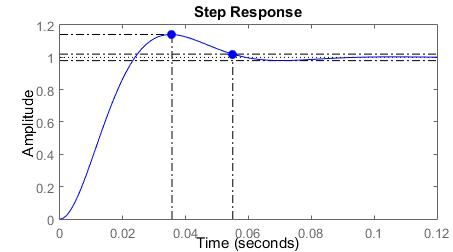
\includegraphics[scale=0.7]{Billeder/PStep.jpg}
\caption{ Peak amplitude: 1.14 - Overshot(\%): 14.1 - At time(seconds): 0.0356
		 Settling time (seconds): 0.055 }
\label{fig:PStep}
\end{figure}

\subsection{Proportional-Integral Controller}

The PI controller accumulates past error terms over time to eliminate steady-state errors in the system. This can cause an increase in overshoot called the integrator wind up, and an increase in settling time. Tough if a requirement is complying a steady-state error of 0, then it is up to the designer to decide, if reaching state-state is more vital to the system, than having more overshot and a longer settling time.\par

Using a PI controller is the same as adding a pole and a zero to the open-loop transfer function. As seen in figure \ref{fig:RlocusControllers}, this controller does not seem to live up to the requirements either. Placing the zero and pole differently could make a better controller, but it would never be able to adjust to both design criterias.\par

The step response of the PI controller is seen on figure \ref{fig:PIStep}, the only difference from the P controller is a slightly longer peak time and settling time and a larger overshoot, as expected. This controller would not meet the requirements. 

\begin{figure}[h!]
\centering
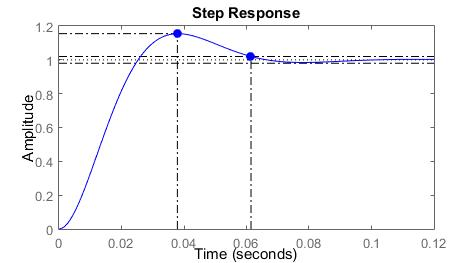
\includegraphics[scale=0.7]{Billeder/PIStep.jpg}
\caption{ Peak amplitude: 1.15 - Overshot(\%): 15.5 - At time(seconds): 0.0379
		 Settling time (seconds): 0.0614 }
\label{fig:PIStep}
\end{figure}

\subsection{Proportional-Derivative Controller}

A PD controller is equivalent to the addition of a simple zero, \textbf{INSERT EQUATION HERE}, which improves the transient response. From a different point of view, the PD controller may also be used to improve the settling time or stability, because it anticipates large errors and attempts corrective action before they occur. 

FIGURE5 shows a promising root locus of the PD controller, it seems like that with the right amount of gain the system would fulfill the requirements.

The step response on figure \ref{fig:PDStep} shows, that in fact this controller would be ideal for this project. There is no overshot, and the settling time is well below 0.05 seconds.

\begin{figure}[h!]
\centering
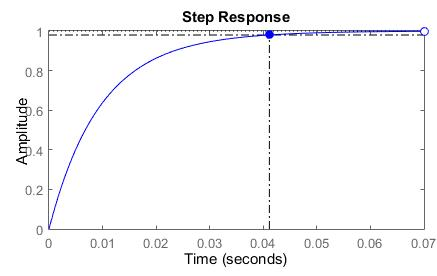
\includegraphics[scale=0.7]{Billeder/PDStep.jpg}
\caption{ Peak amplitude: $>$= 0.998 - Overshot(\%): 0 - At time(seconds): $>$ 0.07
		 Settling time (seconds): 0.0411 }
\label{fig:PDStep}
\end{figure}

\subsection{Proportional-Integral-Derivative Controller}

The PID controller is the most complex controller which is going to be discussed. As noted earlier an PD controller was sufficient for a controller. So why discuss the PID? The reason is that, in reality systems might have limitations which analysis have not taken into account yet. Reaching a steady-state error of 0 is actually a problem with a PD controller for this project, since the pan and tilt system does not function below a certain range of voltage, which means that an integral is needed.\par

Notice on figure \ref{fig:RlocusControllers}, that an PID controller is the addition of 2 zeros and 1 pole to the open-loop transfer function. The root locus shows that this system with a relative gain still meets the requirements of the design.\par

The step response of the PID controller, figure \ref{fig:PIDStep}, shows that indeed a PID controller would be a good choice of controller for this project. There is well below 10\% overshot and the settling time is a great deal below 0.05 seconds.

\begin{figure}[h!]
\centering
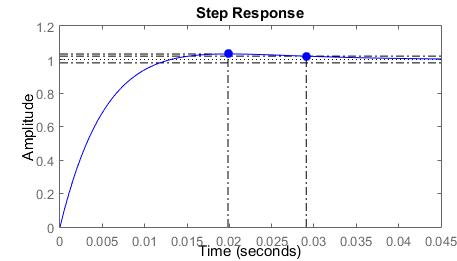
\includegraphics[scale=0.7]{Billeder/PIDStep.jpg}
\caption{ Peak amplitude: 1.03 - Overshot(\%): 2.92 - At time(seconds): 0.0201
		 Settling time (seconds): 0.0277 }
\label{fig:PIDStep}
\end{figure}

\begin{figure}[h!]
\centering
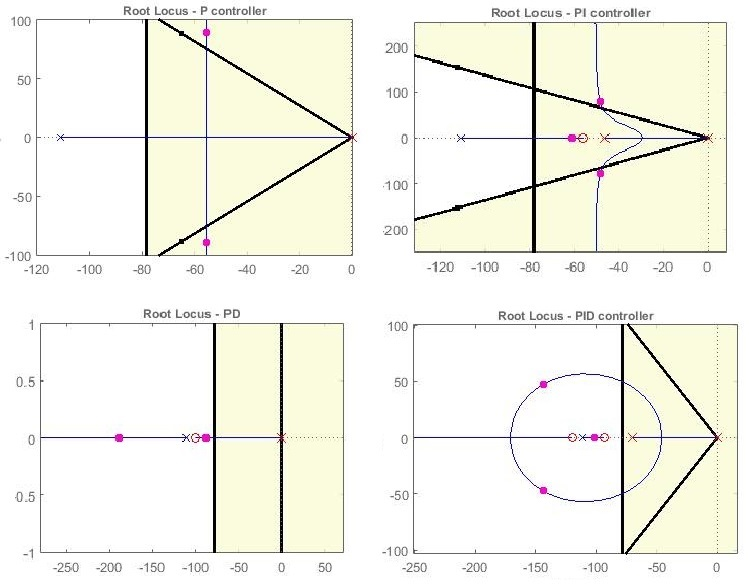
\includegraphics[scale=0.7]{Billeder/RlocusControllers.jpg}
\caption{ Open-loop transfer function Root Locus plots of the estimated motor transfer function, EQUATION REF, with different controllers. The shaded areas indicates designs not met if poles of the closed-loop transfer function is placed there. 
The designs are: Overshot $>$ 10\%, settling time < 0.05 seconds. 7 }
\label{fig:RlocusControllers}
\end{figure}






























